\documentclass[a5paper]{article}
\usepackage[a5paper, top=8mm, bottom=8mm, left=8mm, right=8mm]{geometry}

\usepackage{polyglossia}
\setdefaultlanguage[babelshorthands=true]{russian}

\usepackage{fontspec}
\setmainfont{FreeSerif}
\newfontfamily{\russianfonttt}[Scale=0.7]{DejaVuSansMono}

\usepackage[font=scriptsize]{caption}

\usepackage{amsmath}
\usepackage{amssymb,amsfonts,textcomp}
\usepackage{color}
\usepackage{array}
\usepackage{hhline}
\usepackage{cite}

\usepackage[hang,multiple]{footmisc}
\renewcommand{\footnotelayout}{\raggedright}

\PassOptionsToPackage{hyphens}{url}\usepackage[xetex,linktocpage=true,plainpages=false,pdfpagelabels=false]{hyperref}
\hypersetup{colorlinks=true, linkcolor=blue, citecolor=blue, filecolor=blue, urlcolor=blue, pdftitle=1, pdfauthor=, pdfsubject=, pdfkeywords=}

\usepackage{tabu}

\usepackage{graphicx}
\usepackage{indentfirst}
\usepackage{multirow}
\usepackage{subfig}
\usepackage{footnote}
\usepackage{minted}

\sloppy
\pagestyle{plain}

\title{Domain-Driven Design, стратегические аспекты}
\author{Юрий Литвинов\\\small{yurii.litvinov@gmail.com}}

\date{}

\begin{document}

\maketitle
\thispagestyle{empty}

\section{Целостность модели}

Центральной идеей методологии предметно-ориентированного проектирования является единая модель предметной области и единый язык, что хорошо и правильно, но если над проектом работает сотня человек, это проблематично. Собрать всех на одной кухне, чтобы они могли оттачивать единый язык, физически невозможно, особенно если они на самом деле говорят на разных языках и сидят на разных континентах. В этой лекции речь пойдёт о том, как применять предметно-ориентированное проектирование к проектам, разрабатывающимся несколькими командами, о том, как вообще разрабатывать большие проекты, какие архитектурные проблемы при этом появляются и как их можно решать. Эта лекция по сути является кратким пересказом части IV книги <<Предметно-ориентированное проектирование (DDD). Структуризация сложных программных систем>>, Э. Эванс, и заканчивает рассказ о книге.

Итак, предметно-ориентированное проектирование в случае проекта, над которым работают несколько команд, сталкивается с проблемой того, что команды неизбежно имеют разные видения продукта. Эту проблему можно решать, 

\begin{itemize}
    \item либо поддерживая модель интегрированной --- но тогда затраты на поддержание её целостности будут слишком велики (в идеале --- все команды должны будут непосредственно общаться со всеми остальными, и каждое изменение в модели утверждаться остальными командами), при этом модель наверняка получится слишком общей, чтобы быть полезной;
    \item либо приняв ситуацию как должное и разрешив модели быть фрагментированной --- но тогда это неизбежно затруднит переиспользование кода в рамках проекта и интеграцию системы.
\end{itemize}

При этом бесконтрольное существование модели может привести к ошибкам, связанным с разным пониманием командами нюансов сущностей модели. Эрик Эванс приводил в книжке хороший пример, когда над системой работало несколько команд, и одной из них потребовалась абстракция для платежа клиента. Оказалось, что в коде уже был класс <<Платёж>>, разработанный другой командой, ну и, понятно, его решили переиспользовать. Парочки полей не хватало, одно называлось не совсем так, как надо, но ладно, в конце концов, какое имеет значение конкретное название. Однако система через пару дней начала внезапно падать, в модуле оплаты счетов субподрядчику, для которого изначально был разработан класс <<Платёж>>, в частности, на генерации налоговых отчётов. Стали разбираться, обнаружили в системе странные платежи, которые никто не вводил и которые не имели никакого смысла. Оказалось, что система крешилась из-за того, что у странных платежей не было заполнено поле <<необлагаемый процент>>, несмотря на то, что система требовала его заполнености и сама подставляла туда значение по умолчанию при создании платежа. Выяснилось, что это действительно были платежи клиентов, и для них действительно поле <<необлагаемый процент>> не имело смысла, поэтому просто не заполнялось. И эти платежи тоже попадали в вычисление налоговой отчётности (потому что они платежи же!) и всё падало.

Это выглядит как какая-то частная проблема, но корень зла тут вполне системный --- две команды использовали одну сущность в разных, хоть и похожих, смыслах. И не имели никакого механизма, позволявшего выявить заранее несоответствие значений, которые команды вкладывали в термин <<Платёж>>. Решением проблемы стало создание двух отдельных абстракций <<Платёж поставщику>> и <<Платёж клиента>> и договорённость более не мешать друг другу.

\subsection{Ограниченный контекст}

Командам из примера про <<Платёж>> могла бы помочь заранее достигнутая договорённость о границах их предметных областей и правилах переиспользования кода. В предметно-ориентированном проектировании для этого вводится понятие \textit{<<Ограниченный контекст>>}. Ограниченный контекст (Bounded context) --- это кусок предметной области (и, соответственно, реализующего её кода), в которой применима единая модель предметной области. Всё, что внутри ограниченного контекста, должно следовать этой единой модели, иметь единый язык и т.п., всё, что вне --- не должно делать никаких предположений о модели и не имеет право её без спроса переиспользовать. То есть, ограниченный контекст --- это что-то вроде атомарной области проекта, над которой работает одна команда (как клетка в живом организме, простите за банальную метафору). Разделение системы на ограниченные контексты обычно следует организационной структуре проекта, которая, в свою очередь, чаще всего следует высокоуровневой структуре системы. Например, в одном из проектов, в котором работал автор, по созданию средства автоматизированного реинжиниринга, была группа синтаксического анализа, группа извлечения бизнес-правил, группа генерации кода. Каждая группа имела собственный ограниченный контекст, свою терминологию и своё видение задачи, и интегрировалась с другими с помощью вполне определённых интерфейсов. Что происходило внутри, было делом каждой команды --- например, группа извлечения бизнес-правил занималась вообще какими-то магическими алгоритмами статического анализа программ, которые никто, кроме них, не понимал.

Внутри одного ограниченного контекста может работать довольно большое количество людей, между которыми также может возникнуть недопонимание, напряжение при попытке поддержания единого видения и т.п. Практика показывает, что 3-4 человека, тесно работая вместе, обычно могут договориться, но делить систему на ограниченные контексты по 3-4 человека оказывается непрактично. Поэтому в рамках ограниченного контекста практикуют \textit{<<непрерывную интеграцию>>} в её классическом понимании --- слияние изменений в основную ветку раз в несколько часов, постоянную (после каждого коммита) сборку и запуск юнит-тестов, обеспечение высокого тестового покрытия, непрерывное общение в рамках команды. Всё это позволяет быстро понять наличие проблем в понимании модели внутри ограниченного контекста и устранить их.

Для интеграции с другими ограниченными контекстами могут использоваться \textit{<<карты контекстов>>} (Context map). Карта контекстов фиксирует, как понятие из одной модели в рамках одного ограниченного контекста транслируется в понятие из другой модели из другого контекста. Карты трансляции обычно просто описываются на естественном языке (с применением терминов единых языков интегрируемых моделей), но могут и использоваться диаграммы такого примерно вида:

\begin{center}
    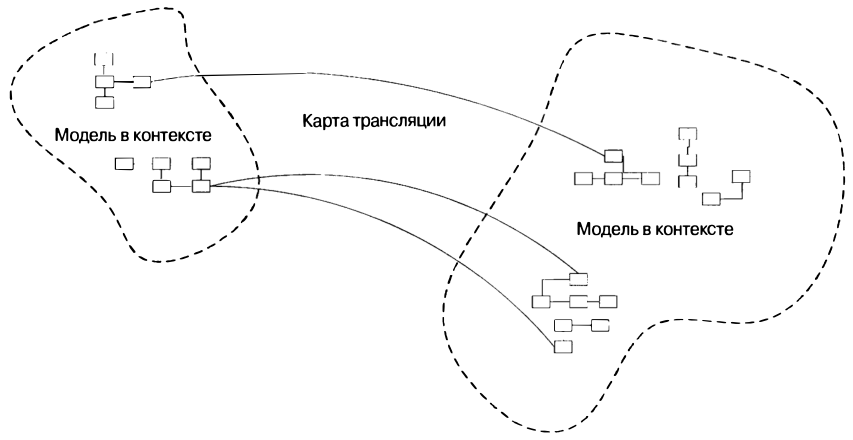
\includegraphics[width=0.7\textwidth]{contextMap.png}
\end{center}

Вот любимый Эриков Эвансом пример про сервис грузоперевозок, показывающий взаимосвязь ограниченных контекстов в рамках одной задачи: 

\begin{center}
    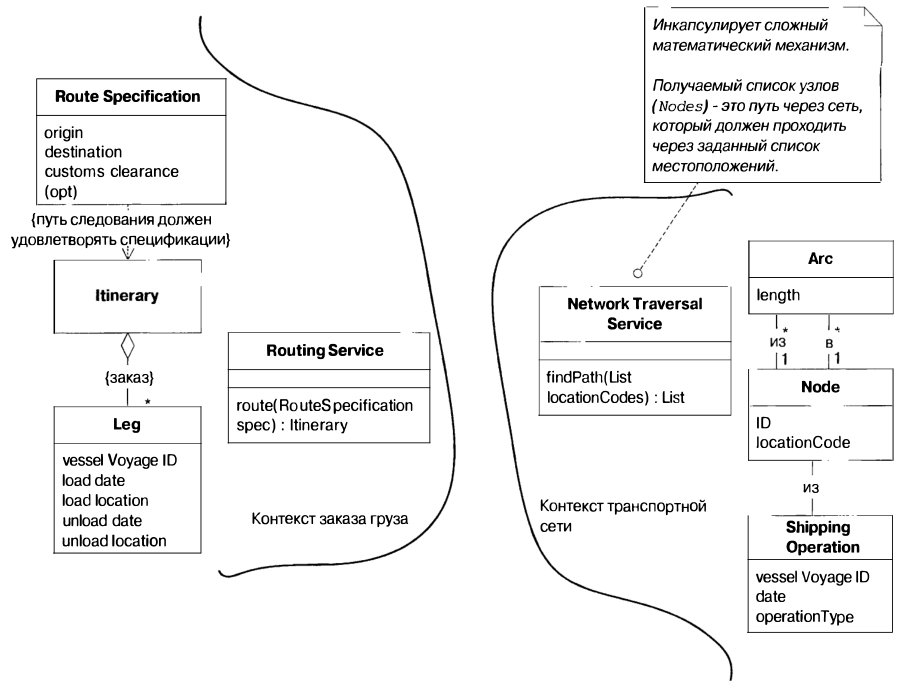
\includegraphics[width=0.8\textwidth]{contextBoundariesExample.png}
\end{center}

Есть команда, занимающаяся бизнес-логикой сервиса прокладки маршрута. Она оперирует понятиями <<Спецификация маршрута>>, <<Маршрут>>, <<Перевозка>> и использует <<Сервис прокладки маршрута>> для вызова кода второй команды, который собственно составляет маршрут перевозки между двумя точками. Вторая команда работает в терминах алгоритмов на графах, она ничего не знает и не хочет знать про перевозки, спецификации маршрута и конкретные корабли или поезда, везущие грузы. У них есть узлы и дуги с весами, узлы привязаны к координатам на местности и в узлах можно осуществлять погрузочно-разгрузочные операции над некоторыми абстрактными транспортными средствами, идентифицируемыми своим кодом. Это позволяет второй команде переиспользовать существующие библиотечные реализации графов и алгоритмов на них, не мучаясь со спецификой предметной области. Но это, естественно, требует определённых усилий на интеграцию, поскольку <<Сервис прокладки маршрута>> со стороны первой команды должен выполнять трансляцию в термины <<Сервиса поиска пути>> второй команды и обратно, и о том, как работают эти сервисы, команды должны чётко договориться. Зато всё, что находится за этими сервисами, может разрабатываться независимо. Что, конечно, приводит к дубликации кода, потому что Leg и Arc, по сути, выражают одно и то же понятие, но в данном случае это абсолютно осмысленно --- команды могут работать параллельно, не мешать друг другу и не мешать разные понятия в одну кучу.

\end{document}